%!TEX root = ../main.tex
\section{Interface}
Interfacet som befinder sig på kasseapparatet, kan som udgangspunkt ligne skitsen som ses her på figur \ref{fig:Interface1}. Dette Interface skal befinde sig på en touchskærm.

\begin{figure}[ht]
	\centering
	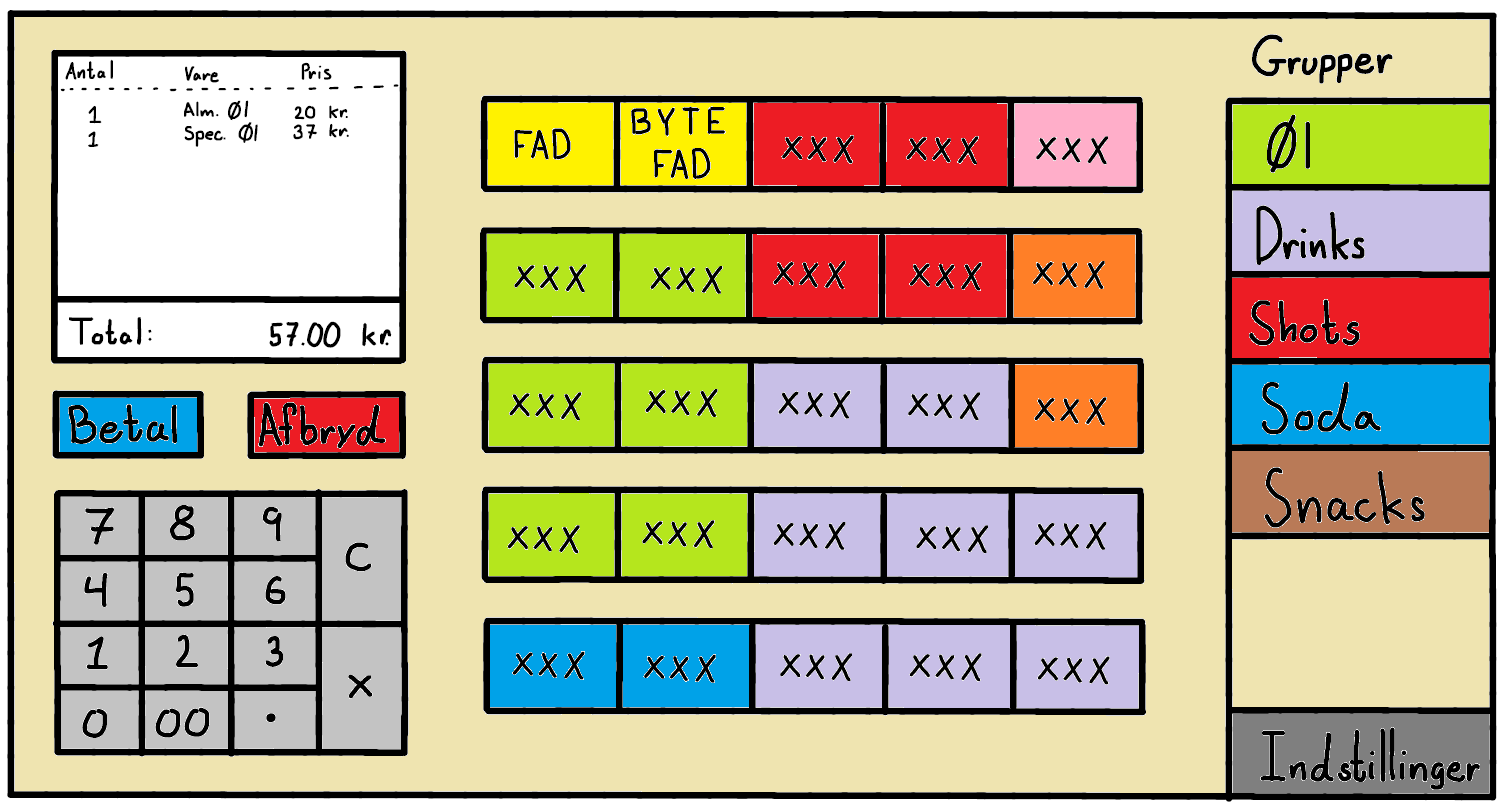
\includegraphics[width=0.8\textwidth]{Kravspecifikation/Interface/Interface1F.png}
	\caption{Skitse for Brugerinterface på kasseapparetet - grupper}
	\label{fig:Interface1}
\end{figure}

For at give Bartenderen mulighed for at lave en hurtig betjening, skal alle valg kunne tages på samme skærmbillede, denne mulighed kan tages under grupper, som ses på figur \ref{fig:Interface1}. 
\newline\newline
På skærmen kan bartenderen se en knap til hver varer, det kunne f.eks. være ''FAD'' for fadøl. Når bartenderen trykker på en vare vil den opstå på varelisten og den totale pris vil blive opdateret. 

\begin{figure}[H]
	\centering
	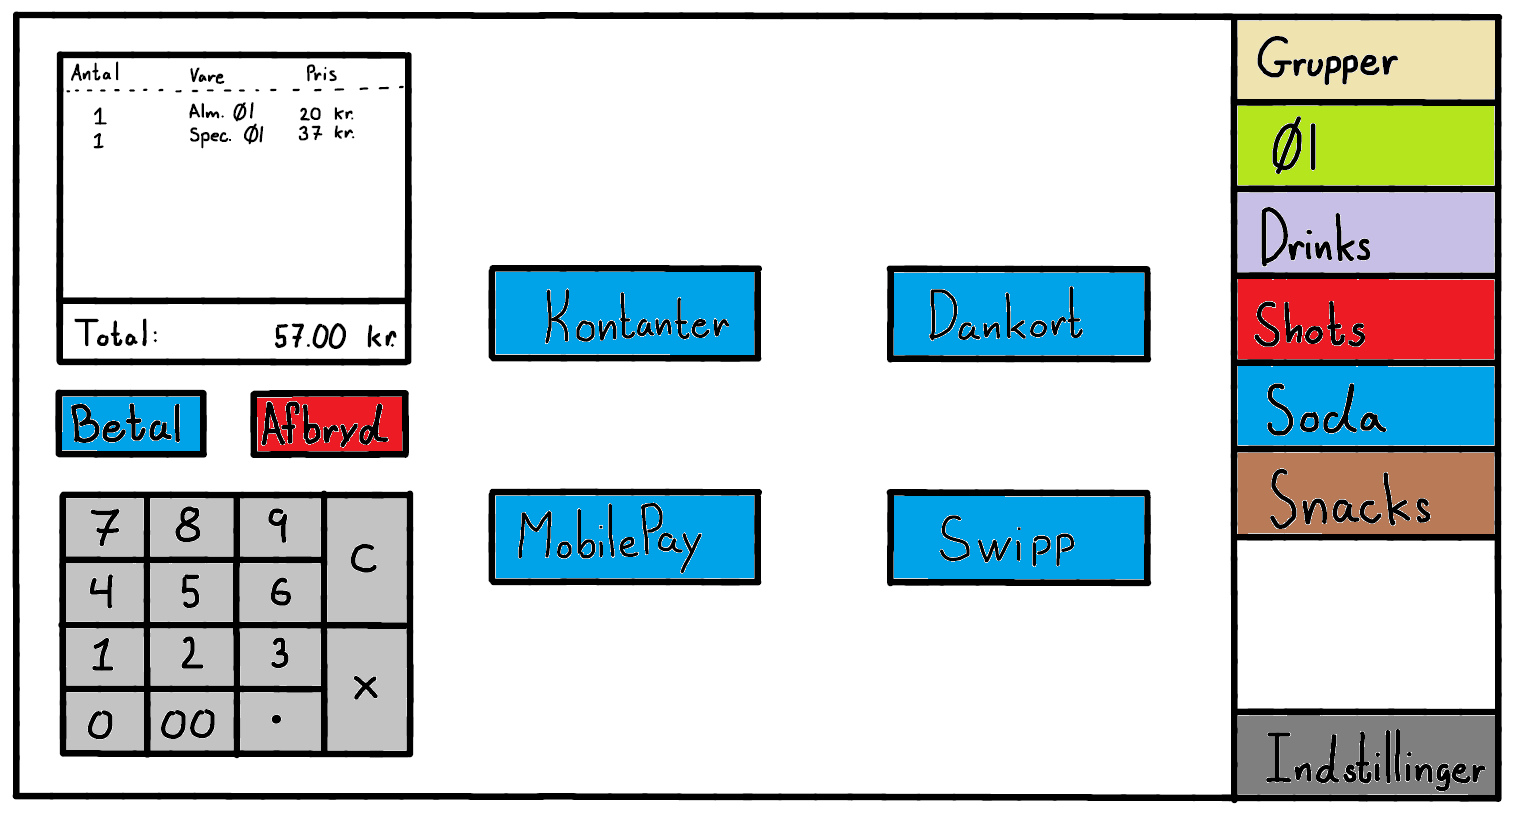
\includegraphics[width=0.8\textwidth]{Kravspecifikation/Interface/Interface3F.png}
	\caption{Skitse for Brugerinterface på kasseapparetet - betaling}
	\label{fig:Interface3}
\end{figure}
Når købet er slut kan bartenderen trykke ''Betal'' som tilgår det skærmbillede, med betalingsmulighederne, som ses på figur \ref{fig:Interface3}. Her trykker bartenderen på den betalingsform der bliver betalt med. 
\newpage
I tilfælde af at bartenderen ønsker nogle mere præcise data om salget, det kunne f.eks. være på dage der ikke er så travlt, kan han vælge at taste den specifikke vare ind, som kan findes under de forskellige kategori ude i højreside af interfacet. Et eksempel på dette kunne f.eks. være ''Øl'', som ses på figur \ref{fig:Interface2}

\begin{figure}[ht]
	\centering
	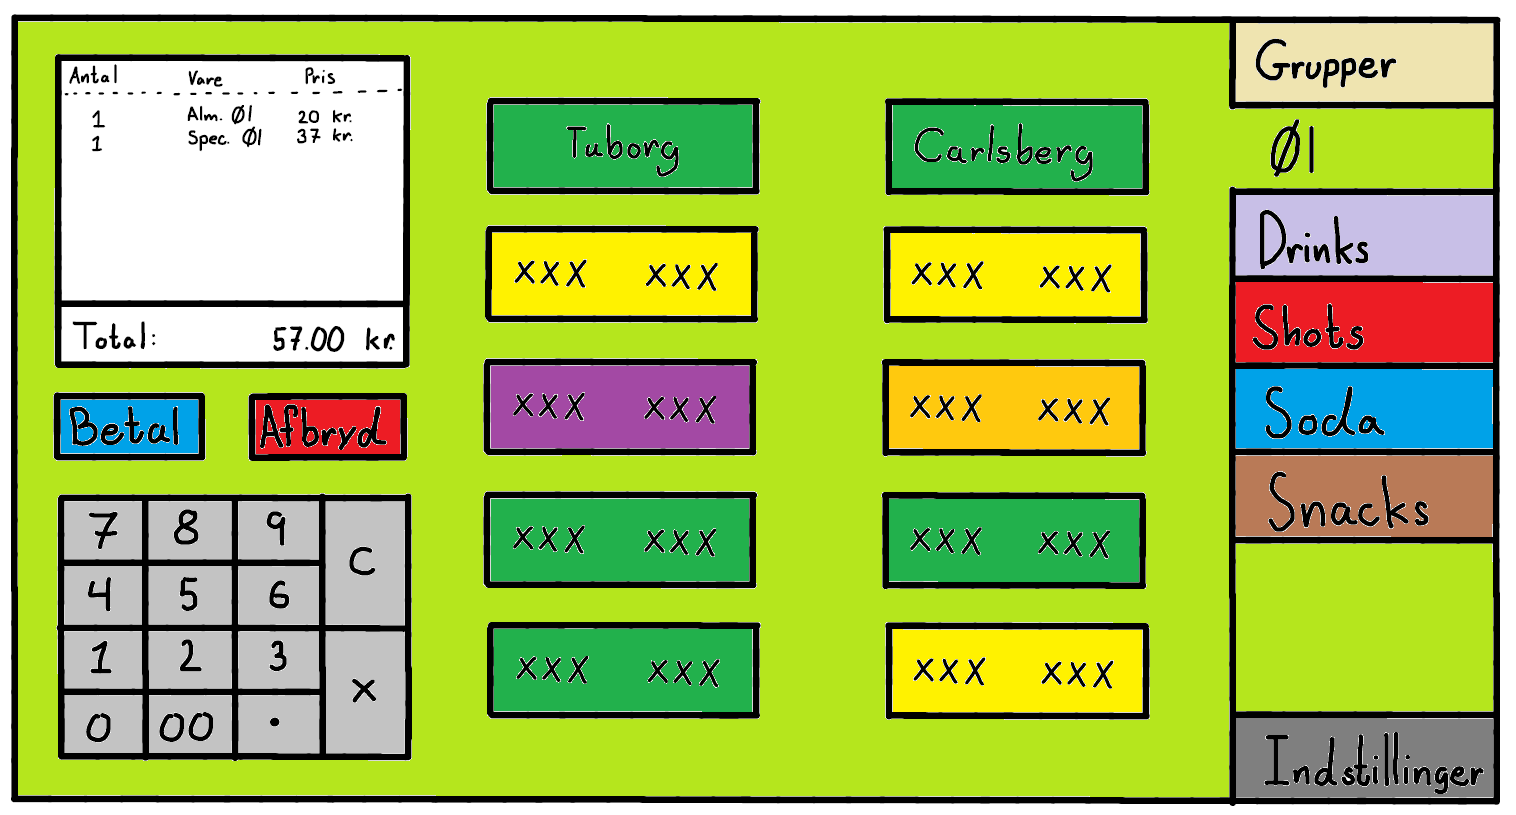
\includegraphics[width=0.8\textwidth]{Kravspecifikation/Interface/Interface2F.png}
	\caption{Skitse for Brugerinterface på kasseapparetet - Øl}
	\label{fig:Interface2}
\end{figure}

Her kan bartenderen så vælge en specifik øl, som f.eks. Tuborg, i stedet for at indtaste alm. øl eller en special øl.

